\PassOptionsToPackage{unicode=true}{hyperref} % options for packages loaded elsewhere
\PassOptionsToPackage{hyphens}{url}
%
\documentclass[]{article}
\usepackage{lmodern}
\usepackage{amssymb,amsmath}
\usepackage{ifxetex,ifluatex}
\usepackage{fixltx2e} % provides \textsubscript
\ifnum 0\ifxetex 1\fi\ifluatex 1\fi=0 % if pdftex
  \usepackage[T1]{fontenc}
  \usepackage[utf8]{inputenc}
  \usepackage{textcomp} % provides euro and other symbols
\else % if luatex or xelatex
  \usepackage{unicode-math}
  \defaultfontfeatures{Ligatures=TeX,Scale=MatchLowercase}
\fi
% use upquote if available, for straight quotes in verbatim environments
\IfFileExists{upquote.sty}{\usepackage{upquote}}{}
% use microtype if available
\IfFileExists{microtype.sty}{%
\usepackage[]{microtype}
\UseMicrotypeSet[protrusion]{basicmath} % disable protrusion for tt fonts
}{}
\IfFileExists{parskip.sty}{%
\usepackage{parskip}
}{% else
\setlength{\parindent}{0pt}
\setlength{\parskip}{6pt plus 2pt minus 1pt}
}
\usepackage{hyperref}
\hypersetup{
            pdfborder={0 0 0},
            breaklinks=true}
\urlstyle{same}  % don't use monospace font for urls
\usepackage{graphicx,grffile}
\makeatletter
\def\maxwidth{\ifdim\Gin@nat@width>\linewidth\linewidth\else\Gin@nat@width\fi}
\def\maxheight{\ifdim\Gin@nat@height>\textheight\textheight\else\Gin@nat@height\fi}
\makeatother
% Scale images if necessary, so that they will not overflow the page
% margins by default, and it is still possible to overwrite the defaults
% using explicit options in \includegraphics[width, height, ...]{}
\setkeys{Gin}{width=\maxwidth,height=\maxheight,keepaspectratio}
\setlength{\emergencystretch}{3em}  % prevent overfull lines
\providecommand{\tightlist}{%
  \setlength{\itemsep}{0pt}\setlength{\parskip}{0pt}}
\setcounter{secnumdepth}{0}
% Redefines (sub)paragraphs to behave more like sections
\ifx\paragraph\undefined\else
\let\oldparagraph\paragraph
\renewcommand{\paragraph}[1]{\oldparagraph{#1}\mbox{}}
\fi
\ifx\subparagraph\undefined\else
\let\oldsubparagraph\subparagraph
\renewcommand{\subparagraph}[1]{\oldsubparagraph{#1}\mbox{}}
\fi

% set default figure placement to htbp
\makeatletter
\def\fps@figure{htbp}
\makeatother


\date{}

\begin{document}

\hypertarget{tutorial-question-and-additional-work}{%
\section{tutorial question and additional
work}\label{tutorial-question-and-additional-work}}

\hypertarget{chapter-1}{%
\subsection{chapter 1}\label{chapter-1}}

section 1.1-1.3

self test 1.1

self test1.2

read 1.3d-1.3g

\hypertarget{section-one-general-review}{%
\section{section one general review}\label{section-one-general-review}}

\hypertarget{quantum-numbers}{%
\subsection{Quantum numbers}\label{quantum-numbers}}

\hypertarget{introduction}{%
\subsubsection{Introduction}\label{introduction}}

Orbitals are a spacial distribution of electron density.All energy
states of electrons within atoms are negative by convention, (as the are
considered to be the minimum energy necessary to free that electron from
its parent atom)

\hypertarget{principle-quantum-number}{%
\subsubsection{principle quantum
number}\label{principle-quantum-number}}

n

\hypertarget{range}{%
\paragraph{range}\label{range}}

\(n \in \mathbb{Z}^+| n \geq 1\)

NOTE: although n is theoretically unbounded values greater than five
have not yet been observed in reality.

\hypertarget{details}{%
\paragraph{details}\label{details}}

Identifies a specific energy state Orbitals of the same quantum number
form an part of the same electron shell

\hypertarget{azimuthal-quantum-number-orbital-angular-momentum-number}{%
\subsubsection{Azimuthal quantum number (orbital angular momentum
number)}\label{azimuthal-quantum-number-orbital-angular-momentum-number}}

l

\hypertarget{encoding}{%
\paragraph{encoding}\label{encoding}}

values of l are given letters for identification

\(\quad 0\rightarrow s\)

\(\quad 1\rightarrow p\)

\(\quad 2\rightarrow d\)

\(\quad 3\rightarrow f\)

\hypertarget{range-1}{%
\paragraph{range}\label{range-1}}

\(l\in \mathbb{Z}\quad | \quad 0 \leq l \leq n-1\quad\)

\hypertarget{details-1}{%
\paragraph{details}\label{details-1}}

determines the size and shape of the sub shell/ determines the area
around the nucleus which the electron may inhabit.

\hypertarget{magnetic-quantum-number}{%
\subsubsection{Magnetic quantum number}\label{magnetic-quantum-number}}

\(m_s\)

\hypertarget{range-2}{%
\paragraph{range}\label{range-2}}

\(m_{l} \in \mathbb{Z} \quad | \quad -l \leq m_{l} \leq l\quad\)

\hypertarget{details-2}{%
\paragraph{details}\label{details-2}}

determines the three dimensional orientation of sub shell.

\hypertarget{spacial-orientations}{%
\paragraph{spacial orientations}\label{spacial-orientations}}

P orbitals have three possible orientations

X,Y,Z

\begin{figure}
\centering
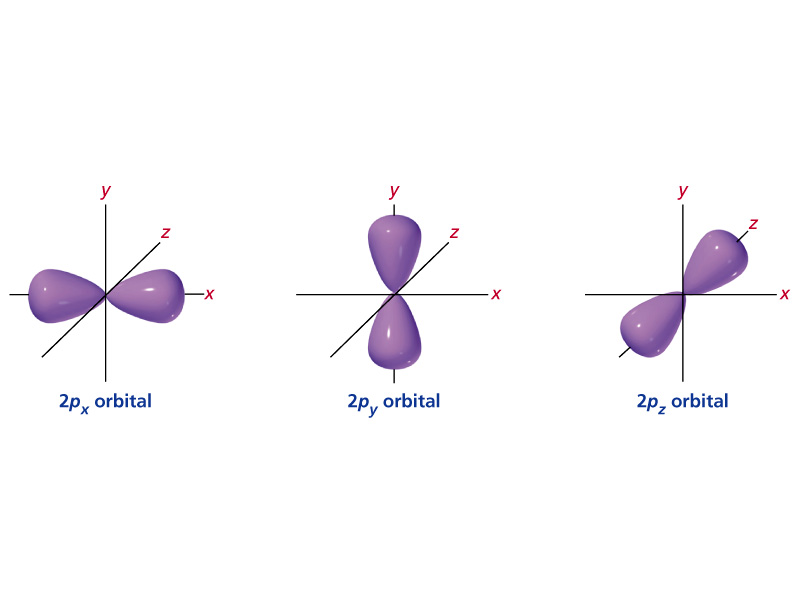
\includegraphics[width=0.5\textwidth,height=\textheight]{Images/dOrbitalOrientation.jpg}
\caption{p orbital orientations}
\end{figure}

D orbitals have five possible orientations

\(xy,xz,zy,z^{2},x^{2}-y^{2}\)

\begin{figure}
\centering
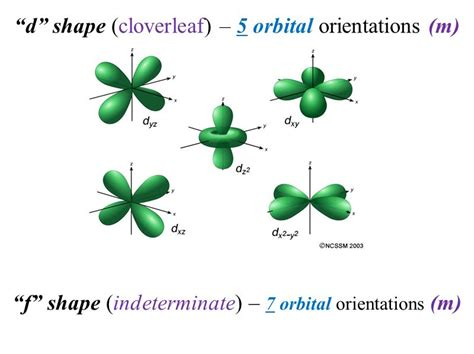
\includegraphics[width=0.5\textwidth,height=\textheight]{Images/dOrbitalOrientations.jpg}
\caption{d orbital orientations}
\end{figure}

F orbitals have seven possible orientations.

\begin{figure}
\centering
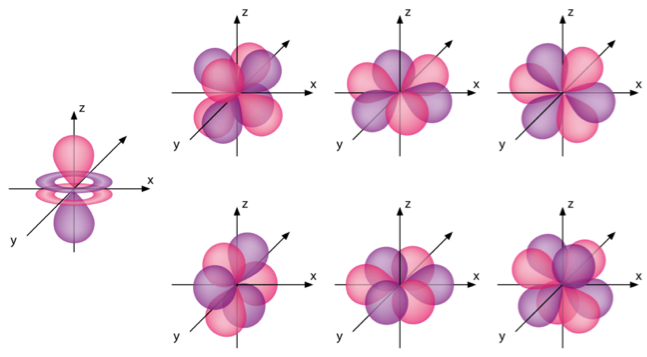
\includegraphics[width=0.5\textwidth,height=\textheight]{Images/fOrbitalOrientations.png}
\caption{forbital orientations}
\end{figure}

\hypertarget{magnetic-spin-number-m_s}{%
\subsubsection{\texorpdfstring{magnetic spin number
\(m_{s}\)}{magnetic spin number m\_\{s\}}}\label{magnetic-spin-number-m_s}}

\hypertarget{range-3}{%
\paragraph{range}\label{range-3}}

\(m_{s} \in \left( \frac{+1}{2},\quad\frac{-1}{2} \right)\)

\hypertarget{details-3}{%
\paragraph{details}\label{details-3}}

determines the direction of spin/ gyration of the electron in regard to
the magnetic axis of the atom.

\hypertarget{representation-diagrams}{%
\subsubsection{representation diagrams}\label{representation-diagrams}}

\hypertarget{standard-representation}{%
\paragraph{Standard representation}\label{standard-representation}}

\(nl^{s}\)

Where:

\begin{verbatim}
  n= principle quantum number
  l= azimuthal number
  x= number of electrons within the l subshell.      
\end{verbatim}

\hypertarget{condensed-representation}{%
\paragraph{Condensed representation}\label{condensed-representation}}

{[}noble gases{]} valence shell in standard representation

\hypertarget{pauli-exclusion-principles.}{%
\subsubsection{Pauli Exclusion
Principles.}\label{pauli-exclusion-principles.}}

no too electron within one atom can have the same set of quantum numbers

\hypertarget{effective-nuclear-charge}{%
\subsection{Effective nuclear charge}\label{effective-nuclear-charge}}

effective nuclear charge is the charge exerted on a given electron
within an atom by the (positively charged) nucleus of that atom

\hypertarget{shielding}{%
\subsubsection{shielding}\label{shielding}}

shielding is the reduction of the full nuclear charge which and in
isolation the nucleus would exert on an electron.

\(Z_{eff} = Z - \sigma\quad\)

where: \(Z_{eff}\) = effective nuclear charge Z= nuclear charge
\(\sigma\) = shielding effect of other electrons.

this shielding effect is due to the present of other electrons within
the atom which repel the electron in question reducing the net
attractive force towards the nucleus which it feels.

(this reduction is often expressed as the reduction of
\(Z \quad to \quad Z_{eff}\) )

\hypertarget{penetration}{%
\subsubsection{penetration}\label{penetration}}

the potential for the presence of an electron inside shells of other
electrons. (?)

\hypertarget{slaters-rules}{%
\subsubsection{Slater's Rules}\label{slaters-rules}}

Estimated value for sigma

\hypertarget{final-electron-is-in-a-s-or-p-orbital}{%
\paragraph{final electron is in a s or p
orbital}\label{final-electron-is-in-a-s-or-p-orbital}}

\begin{itemize}
\tightlist
\item
  n-1 electrons contribute 0.85
\item
  ns and np electrons contribute 0.35 to \(\sigma\quad\)
\item
  n-2 or lower electrons contribute 1.0 to \(\sigma\quad\)
\end{itemize}

\hypertarget{final-electron-is-in-a-d-or-f-orbital}{%
\paragraph{final electron is in a d or f
orbital}\label{final-electron-is-in-a-d-or-f-orbital}}

\begin{itemize}
\tightlist
\item
  nf and nd electrons contribute 0.35 to \(\sigma\quad\)
\item
  electrons in lower shells contribute 1. to \(\sigma\quad\)
\end{itemize}

\hypertarget{trends}{%
\subsubsection{Trends}\label{trends}}

the closer to the nuclear an electron is the smaller the difference
between Z and \(Z_{eff}\) will be.

\end{document}
